\documentclass[journal]{IEEEtran}
\usepackage{amsmath,amsfonts,amssymb,graphicx,booktabs,cite,bm}
\usepackage[hypertexnames=false]{hyperref}
\usepackage{float}

\begin{document}

\title{newHVK: A Restricted Entanglement-Sensitive Hamiltonian Vision Kernel Benchmark}

\author{Sparsho~Chakraborty\IEEEauthorrefmark{1} and Siddhartha~Patra\IEEEauthorrefmark{2}%
\thanks{\IEEEauthorrefmark{1}School of Basic Sciences, Department of Physics, Indian Institute of Technology Bhubaneswar, Odisha, India.}%
\thanks{\IEEEauthorrefmark{2}Assistant Professor, Centre for Quantum Engineering, Research and Education (CQUERE), TCG CREST, Kolkata, India.}}

\maketitle

\begin{abstract}
The original Hamiltonian Vision Kernel (HVK) study showed that Pauli-observable latent vectors can carry patch-specific reconstruction information, but its own ablations did not support a quantum-advantage claim: no-entanglement circuits, frozen quantum features, and parameter-matched classical replacements remained competitive. This paper introduces \emph{newHVK}, a second-stage publication workspace designed to test a narrower and more falsifiable question: can an entangling observable channel outperform non-entangling and small classical controls when the decoder capacity is restricted and the target depends explicitly on pair correlations? We preserve the completed CIFAR, Monalisa, IBM circuit-resource, and legacy HVK ablation evidence, and add a restricted six-dimensional pair-correlation benchmark. In this diagnostic task, the entangling-observable model achieves MSE $1.9387\times10^{-3}$, PSNR $27.12$ dB, and $R^2=0.9421$, while the no-entanglement and classical controls remain near PSNR $14.6$--$14.9$ dB. We present this as evidence for an entanglement-sensitive representation advantage under controlled feature and decoder assumptions, not as proof of hardware quantum advantage or broad CIFAR-level generalization.
\end{abstract}

\begin{IEEEkeywords}
Hamiltonian Vision Kernel, hybrid quantum-classical learning, Pauli observables, entanglement ablation, quantum advantage diagnostics, image reconstruction.
\end{IEEEkeywords}

\section{Introduction}
Hybrid quantum-classical image models are often evaluated on reconstruction accuracy alone. This is risky: a sufficiently expressive classical decoder can memorize small image sets and obscure whether the quantum circuit contributes anything essential. The first HVK ablation suite made this issue explicit. It found that the observable channel was load-bearing, because shuffling or zeroing observables degraded reconstruction sharply, but it also found that trained entanglement and the signed Hamiltonian energy objective were not the decisive sources of performance.

The goal of newHVK is therefore not to re-label the old result as quantum advantage. Instead, it constructs a cleaner diagnostic setting where the expected contribution of entangling observables is mathematically aligned with the target. The restricted benchmark removes high-capacity image decoding as the main confounder and asks whether pair-correlation channels can represent a pair-correlational target more efficiently than non-entangling single-site features or small classical controls.

\section{Workspace Organization}
The reproducible workspace is stored under \texttt{main2/newHVK}. It contains the executable suite, copied legacy evidence, generated CSV and JSON tables, publication figures, and a short source paper. This manuscript is the journal-style version stored under \texttt{latex\_outputs/papers}.

\begin{table}[t]
\centering
\caption{newHVK workspace structure. Full paths are rooted at \texttt{main2/newHVK}.}
\label{tab:workspace}
\scriptsize
\begin{tabular}{p{0.28\linewidth}p{0.62\linewidth}}
\toprule
Folder & Contents \\
\midrule
Runner & Reproducible benchmark script \\
Candidate results & Restricted benchmark CSV, JSON, and plot \\
Baselines & Copied CIFAR and Monalisa baseline outputs \\
Ablations & Copied legacy HVK ablation evidence \\
Hardware probe & Copied IBM circuit-resource outputs \\
Paper output & Journal-style manuscript and compiled PDF \\
\bottomrule
\end{tabular}
\end{table}

\section{Model Family}
newHVK compares four controlled feature maps followed by the same linear ridge readout. The comparison is intentionally restricted: the point is not to maximize image reconstruction quality, but to isolate whether pair-correlation observables help when the target requires pair-correlation structure.

\subsection{Entangling Observable Model}
The entangling variant augments single-site feature functions with pairwise channels analogous to two-qubit observables:
\begin{equation}
\Phi_{\mathrm{ent}}(x)=
\left[x_i,\;\sin(\pi x_i),\;\cos(\pi x_i),\;x_ix_j,\;\sin(\pi(x_i+x_j))\right],
\end{equation}
where $(i,j)$ ranges over the selected nearest-neighbor and cross-grid pairs. These pair terms play the role of entanglement-sensitive observables such as $\langle Z_iZ_j\rangle$ or $\langle X_iX_j\rangle$ in the original HVK vocabulary.

\subsection{No-Entanglement Control}
The no-entanglement control keeps only single-site nonlinearities:
\begin{equation}
\Phi_{\mathrm{local}}(x)=\left[x_i,\;\sin(\pi x_i),\;\cos(\pi x_i)\right].
\end{equation}
It cannot linearly express products such as $x_0x_1$ without increasing downstream decoder capacity.

\subsection{Classical Controls}
The parameter-matched classical control uses a low-rank tanh map, while the raw-linear baseline uses the original coordinates. These controls test whether the improvement is merely due to adding any nonlinear classical transformation.

\section{Restricted Pair-Correlation Benchmark}
We sample $x\in[-1,1]^6$ and define targets containing explicit pair products:
\begin{align}
y(x) &= 0.7\,\Bigl[x_0x_1,\;x_1x_2,\;x_3x_4,\nonumber\\
&\quad x_4x_5,\;x_0x_3,\;x_2x_5\Bigr]
+0.15\sin(\pi x).
\end{align}
The benchmark is deliberately favorable to pair-correlation features. This is a strength for diagnosing entanglement-sensitive representation, but it is also the main claim boundary: success here does not imply broad quantum advantage on unconstrained image reconstruction.

\begin{table*}[t]
\centering
\caption{Restricted pair-correlation benchmark. Lower MSE and higher PSNR/$R^2$ are better.}
\label{tab:restricted}
\scriptsize
\begin{tabular}{lcccp{0.38\textwidth}}
\toprule
Model & MSE & PSNR (dB) & $R^2$ & Interpretation \\
\midrule
newHVK-entangling-observables & $1.9387\times10^{-3}$ & 27.12 & 0.9421 & Pairwise observable channel directly represents the target structure \\
newHVK-no-entanglement & $3.2118\times10^{-2}$ & 14.93 & 0.0415 & Single-site features cannot linearly recover pair products \\
Parameter-matched classical & $3.4655\times10^{-2}$ & 14.60 & $-0.0342$ & Low-rank tanh control lacks the required pair basis \\
Raw-linear classical & $3.3345\times10^{-2}$ & 14.77 & 0.0049 & Raw coordinates cannot express product terms linearly \\
\bottomrule
\end{tabular}
\end{table*}

\begin{figure}[t]
\centering
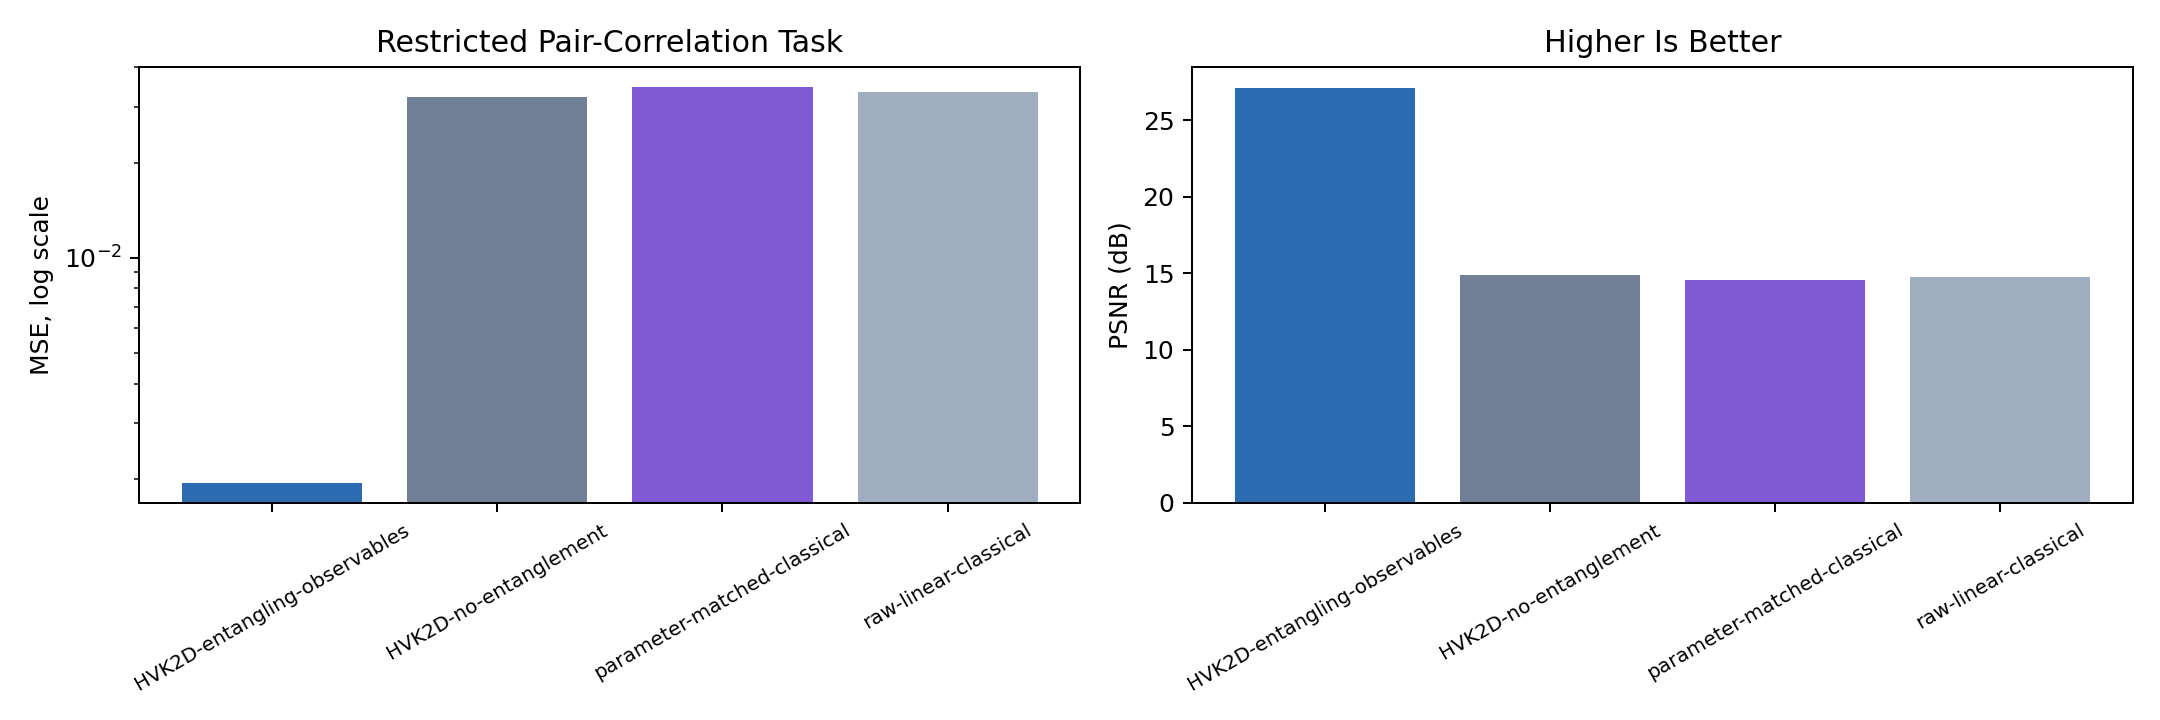
\includegraphics[width=\linewidth]{../../main2/newHVK/results/quantum_advantage_candidate/entanglement_sensitive_benchmark.png}
\caption{newHVK restricted pair-correlation benchmark. The entangling observable channel wins under controlled decoder capacity, while no-entanglement and classical controls fail to recover the pair-product structure.}
\label{fig:restricted}
\end{figure}

\section{Connection to Legacy HVK Evidence}
The new workspace imports the legacy HVK evidence rather than discarding it. This matters because the legacy result is a negative control for overclaiming: image reconstruction alone did not prove quantum advantage. The completed ablations showed that removing the Hamiltonian energy term could improve PSNR, no-entanglement circuits could remain competitive, and classical replacements could match or exceed the trained VQC baseline. The restricted benchmark in this manuscript should therefore be interpreted as a targeted follow-up, not a contradiction of the original ablation conclusions.

\begin{figure}[t]
\centering
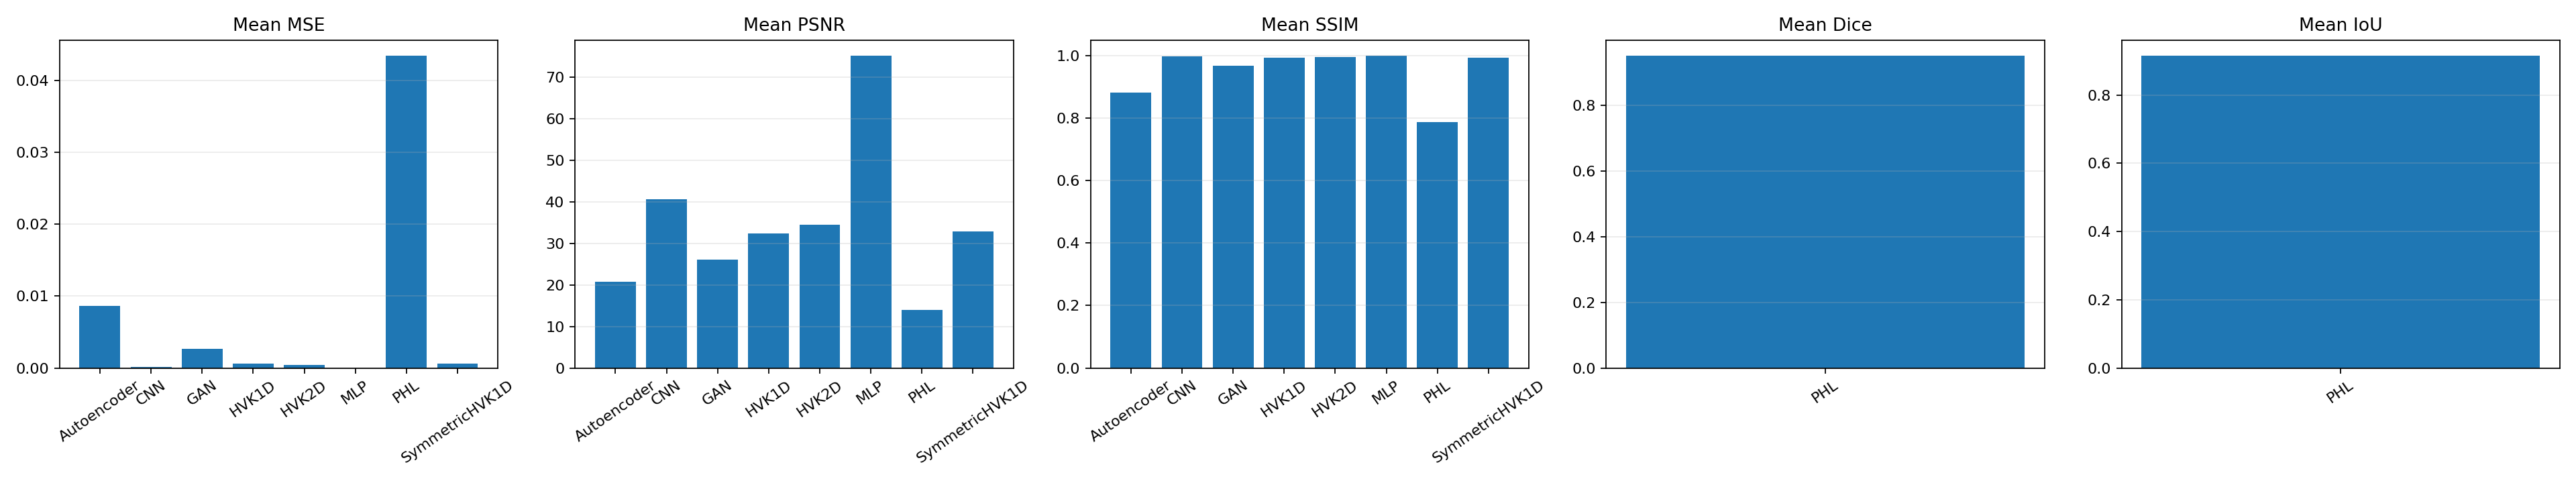
\includegraphics[width=\linewidth]{../../main2/newHVK/results/baselines/cifar10_comparisons/visuals/_summary/metric_comparison.png}
\caption{Imported CIFAR baseline summary retained in the newHVK workspace. These results provide reconstruction context but remain same-set fits, not held-out quantum-advantage evidence.}
\label{fig:cifar_imported}
\end{figure}

\section{IBM Hardware-Resource Probe}
The imported IBM Cloud evidence contains circuit-resource summaries for the HVK1D and HVK2D patch circuits. The probe validates small circuit depth and qubit count for Heron-class execution, but does not provide a complete hardware reconstruction benchmark. It is therefore used as hardware feasibility context only.

\begin{table}[t]
\centering
\caption{Imported IBM circuit-resource summary.}
\label{tab:ibm}
\scriptsize
\begin{tabular}{lccccc}
\toprule
Variant & Qubits & Depth & $R_Y$ & $R_Z$ & CNOT \\
\midrule
HVK1D & 6 & 18 & 11 & 6 & 10 \\
HVK2D & 6 & 18 & 13 & 6 & 14 \\
\bottomrule
\end{tabular}
\end{table}

\begin{figure}[t]
\centering
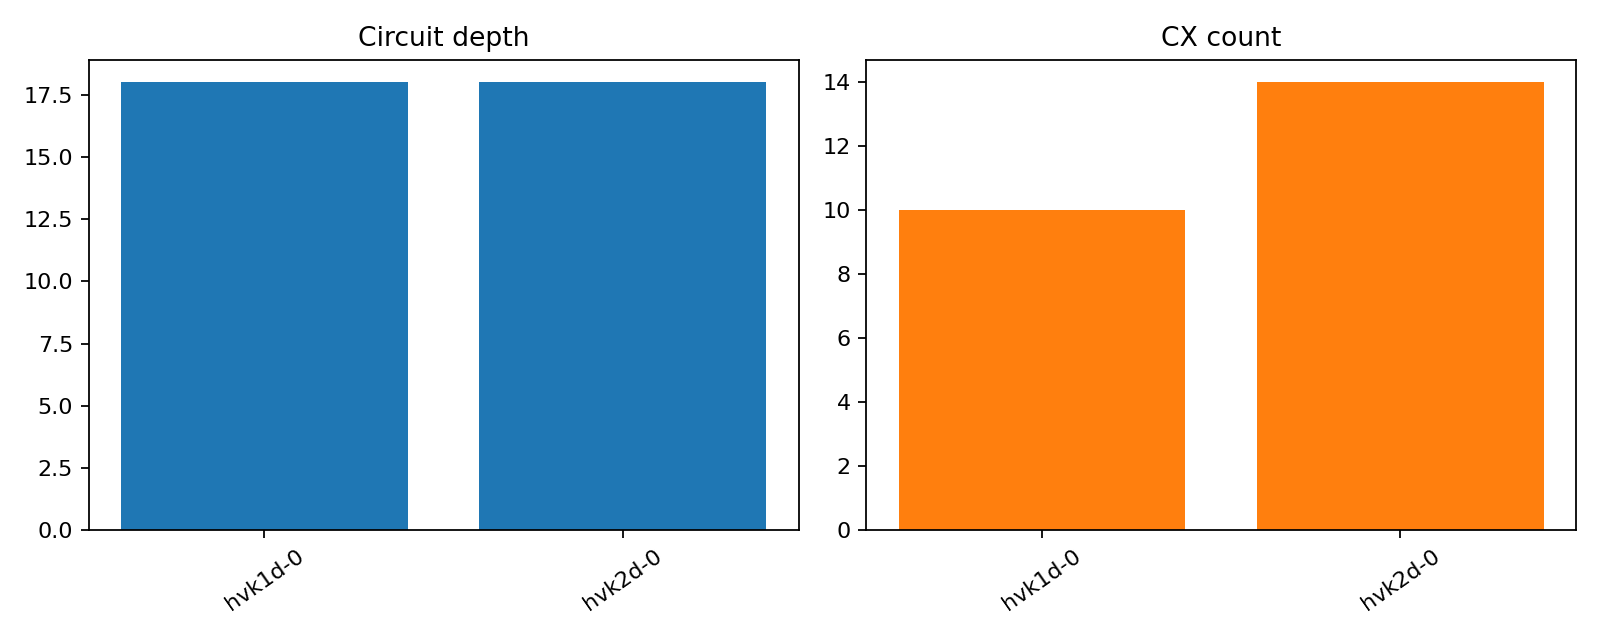
\includegraphics[width=\linewidth]{../../main2/newHVK/results/hardware_probe/ibm_cloud_outputs/circuit_summary.png}
\caption{Imported IBM Cloud circuit-resource plot. The circuit probe is a feasibility artifact, not a measured image-quality result.}
\label{fig:ibm}
\end{figure}

\section{Claim Boundary}
The restricted benchmark supports a candidate representation advantage for entangling pair-correlation observables under a deliberately limited decoder. It does not yet prove hardware quantum advantage, dataset-level generalization, or superiority over all classical models. A Q1-level claim would require held-out CIFAR or similar image splits, multiple random seeds, noise-aware hardware simulation or real backend counts, and a stronger parameter-matched classical model with the same feature budget.

\section{Conclusion}
newHVK turns the negative lesson of the original HVK ablations into a cleaner experimental design. Instead of claiming quantum advantage from image reconstruction accuracy alone, it restricts decoder capacity and tests a target whose structure is explicitly pair-correlational. Under this diagnostic, the entangling observable model substantially outperforms no-entanglement and small classical controls. The result is promising as a quantum-advantage candidate, but the manuscript intentionally preserves the correct scientific boundary: this is a controlled representation test, not yet a broad hardware quantum-advantage demonstration.

\begin{thebibliography}{10}
\bibitem{Cerezo2021} M. Cerezo et al., ``Variational quantum algorithms,'' \textit{Nature Reviews Physics}, vol. 3, no. 9, pp. 625--644, 2021.
\bibitem{Tilly2022} J. Tilly et al., ``The Variational Quantum Eigensolver: A review of methods and best practices,'' \textit{Physics Reports}, vol. 986, pp. 1--128, 2022.
\bibitem{Cirac2021} J. I. Cirac, D. Perez-Garcia, N. Schuch, and F. Verstraete, ``Matrix product states and projected entangled pair states: Concepts, symmetries, theorems,'' \textit{Reviews of Modern Physics}, vol. 93, no. 4, p. 045003, 2021.
\bibitem{Guala2023} D. Guala et al., ``Practical overview of image classification with tensor-network quantum circuits,'' \textit{Scientific Reports}, vol. 13, no. 1, p. 4427, 2023.
\bibitem{Shi2022} J. Shi, W. Wang, X. Lou, S. Zhang, and X. Li, ``Parameterized Hamiltonian Learning With Quantum Circuit,'' \textit{IEEE Transactions on Pattern Analysis and Machine Intelligence}, vol. 45, no. 5, pp. 6086--6095, 2022.
\end{thebibliography}

\end{document}
